\documentclass[12pt,letterpaper]{article}
\usepackage[spanish]{babel}
\usepackage[utf8]{inputenc}
\usepackage{graphicx}
\usepackage{listings}
\usepackage{xcolor}
\usepackage{hyperref}
\usepackage{amsmath}
\usepackage{float}
\usepackage{fancyhdr}
\usepackage{lastpage}
\usepackage{titling}

% Configuración del encabezado y pie de página
\setlength{\headheight}{50pt} % Aumentamos la altura del encabezado para el logo
\addtolength{\topmargin}{-35pt} % Ajustamos el margen superior
\pagestyle{fancy}
\fancyhf{}
\renewcommand{\headrulewidth}{1pt}
\renewcommand{\footrulewidth}{1pt}
\fancyhead[L]{
\includegraphics[height=35pt]{images/logo_uct.png}}
\fancyhead[R]{Programación~II}
\fancyfoot[C]{Página~\thepage~de~\pageref{LastPage}}
\fancyfoot[R]{Octubre~2025}

% Aumentar el espacio superior del título
\setlength{\droptitle}{-4em}

% Configuración de colores y estilo para código
\definecolor{codegreen}{rgb}{0,0.6,0}
\definecolor{codegray}{rgb}{0.5,0.5,0.5}
\definecolor{codepurple}{rgb}{0.58,0,0.82}
\definecolor{backcolour}{rgb}{0.95,0.95,0.92}

\lstdefinestyle{mystyle}{
    backgroundcolor=\color{backcolour},   
    commentstyle=\color{codegreen},
    keywordstyle=\color{magenta},
    numberstyle=\tiny\color{codegray},
    stringstyle=\color{codepurple},
    basicstyle=\ttfamily\footnotesize,
    breakatwhitespace=false,         
    breaklines=true,                 
    captionpos=b,                    
    keepspaces=true,                 
    numbers=left,                    
    numbersep=5pt,                  
    showspaces=false,                
    showstringspaces=false,
    showtabs=false,                  
    tabsize=2
}

\lstset{style=mystyle}

\title{\textbf{Sistema de Gestión de Restaurante}\\
\large Evaluación 2 --- Programación II\\
\vspace{0.5cm}
\normalsize Universidad Católica de Temuco\\
\normalsize Facultad de Ingeniería\\
\normalsize Ingeniería Civil Informática}

\author{
    \textbf{Integrantes:}\\
    \vspace{0.3cm}
    Joaquin Carrasco Duran\\
    \vspace{0.3cm}
    Benjamin Cabrera\\
    \vspace{0.3cm}
    Leonardo Chavez\\
    \vspace{0.3cm}
    \textbf{Profesor:} Guido Mellado\\
    \vspace{0.3cm}
    \textbf{Asignatura:} Programación II\\
    \vspace{0.3cm}
    \textbf{Sección:} 2
}

\date{Octubre 2025}

\begin{document}

\maketitle
\newpage
\tableofcontents
\newpage

\section{Introducción}
Este informe presenta el desarrollo de un sistema de gestión para restaurantes implementado en Python. El sistema permite la administración de inventario, gestión de pedidos, generación de boletas y visualización de menús utilizando una interfaz gráfica moderna con customtkinter.

\section{Objetivos}
\subsection{Objetivo General}
Desarrollar un sistema de gestión integral para restaurantes que permita administrar inventario, pedidos y generación de documentos de manera eficiente.

\subsection{Objetivos Específicos}
\begin{itemize}
    \item Implementar un sistema de gestión de inventario para ingredientes
    \item Crear un sistema de pedidos con interfaz gráfica
    \item Desarrollar un generador de boletas automatizado
    \item Implementar visualización de menús en formato PDF
\end{itemize}

\section{Arquitectura del Sistema}
El sistema está desarrollado siguiendo los principios de la programación orientada a objetos y utiliza varios patrones de diseño para mantener una estructura modular y mantenible.

\subsection{Patrones de Diseño Utilizados}
\begin{itemize}
    \item \textbf{Patrón Facade}: Implementado en la clase BoletaFacade para simplificar la generación de boletas.
    \item \textbf{Protocol (Interfaz moderna)}: Utilizado en IMenu para definir el contrato de los elementos del menú. Se implementa usando el módulo typing.Protocol de Python, que proporciona una forma más flexible y moderna de definir interfaces.
    \item \textbf{Patrón Composite}: Aplicado en la estructura de menús e ingredientes.
\end{itemize}

\section{Diagrama de Clases}
\subsection{Estructura del Sistema}
\begin{figure}[H]
    \centering
    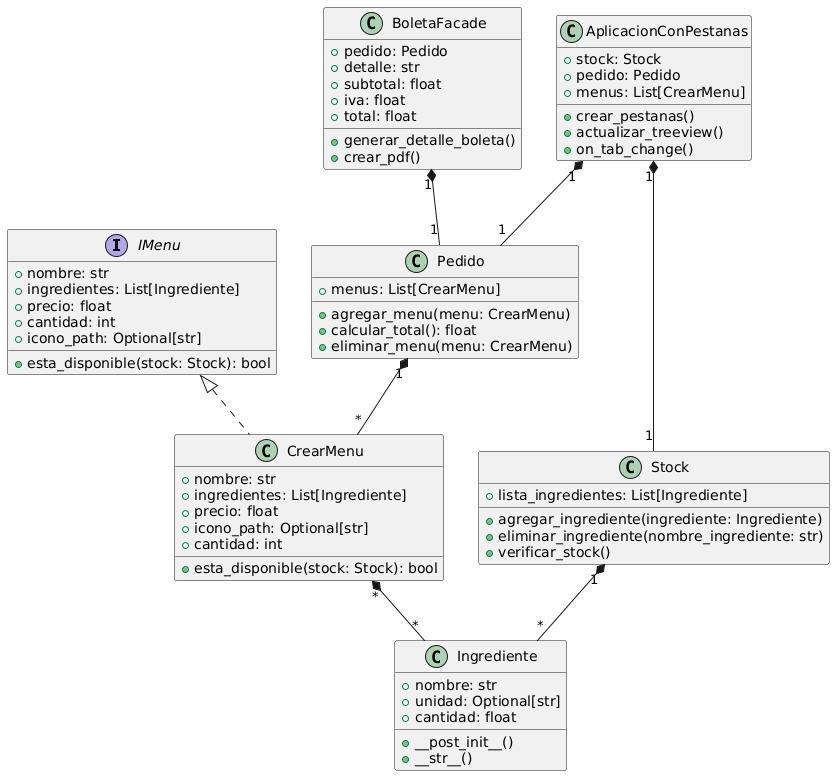
\includegraphics[width=\textwidth]{./images/diagrama.png}
    \caption{Diagrama de Clases del Sistema}\label{fig:diagrama}
\end{figure}

\subsection{Explicación del Diagrama}
\begin{figure}[H]
    \centering
    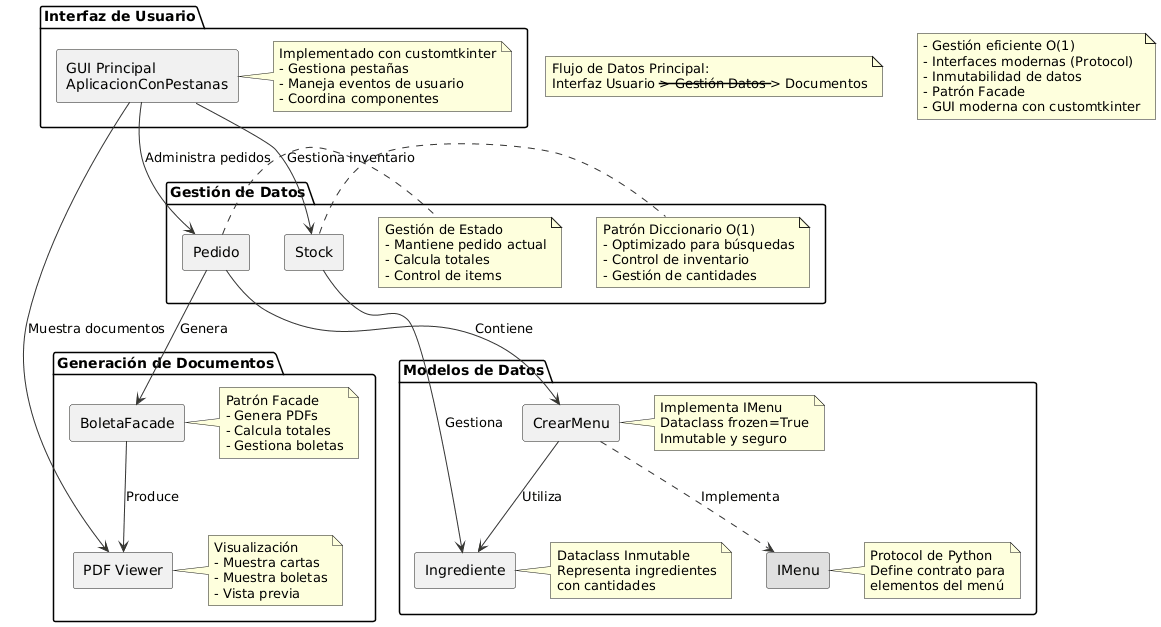
\includegraphics[width=\textwidth]{./images/explicacion_diagrama.png}
    \caption{Explicación Detallada de las Relaciones entre Clases}\label{fig:explicacion-diagrama}
\end{figure}

\subsection{Descripción de las Clases}
\begin{itemize}
    \item \textbf{AplicacionConPestanas}: Clase principal que coordina todas las funcionalidades del sistema.
    \item \textbf{Stock}: Gestiona el inventario de ingredientes.
    \item \textbf{Ingrediente}: Representa los ingredientes individuales.
    \item \textbf{CrearMenu}: Implementa la interfaz IMenu y representa los elementos del menú.
    \item \textbf{Pedido}: Maneja la gestión de pedidos.
    \item \textbf{BoletaFacade}: Simplifica la generación de boletas.
\end{itemize}

\section{Tecnologías Utilizadas}
\begin{itemize}
    \item \textbf{Python 3.13}: Lenguaje de programación principal
    \item \textbf{customtkinter}: Framework para la interfaz gráfica moderna
    \item \textbf{FPDF}: Biblioteca para generación de PDFs
    \item \textbf{PyMuPDF (fitz)}: Visualización de PDFs
    \item \textbf{Pandas}: Procesamiento de datos CSV
\end{itemize}

\section{Implementación}
\subsection{Gestión de Inventario}
El sistema maneja el inventario a través de la clase Stock, que utiliza un diccionario (de tipo Dict[str, Ingrediente]) como estructura de datos principal. Esta decisión de diseño garantiza un rendimiento óptimo con complejidad $O(1)$ para todas las operaciones principales:

\begin{itemize}
    \item Agregar nuevos ingredientes
    \item Eliminar ingredientes existentes
    \item Verificar disponibilidad
    \item Actualizar cantidades
\end{itemize}

A continuación, se muestra un ejemplo de la implementación del manejo de stock:

\begin{lstlisting}[language=Python, caption=Implementación de Stock]
class Stock:
    def __init__(self):
        self.lista_ingredientes: Dict[str, Ingrediente] = {}

    def agregar_ingrediente(self, ingrediente: Ingrediente):
        if ingrediente.nombre in self.lista_ingredientes:
            ing_existente = self.lista_ingredientes[ingrediente.nombre]
            nueva_cantidad = ing_existente.cantidad + ingrediente.cantidad
            ing_existente.cantidad = round(nueva_cantidad, 1)
        else:
            ingrediente.cantidad = round(ingrediente.cantidad, 1)
            self.lista_ingredientes[ingrediente.nombre] = ingrediente

    def verificar_ingredientes_suficientes(self, 
            ingredientes_necesarios: List[Ingrediente]) -> bool:
        for ing_necesario in ingredientes_necesarios:
            ing_stock = self.lista_ingredientes.get(ing_necesario.nombre)
            if ing_stock is None or ing_stock.cantidad < ing_necesario.cantidad:
                return False
        return True
\end{lstlisting}

\subsection{Sistema de Pedidos}
La gestión de pedidos se realiza mediante la clase Pedido, que ofrece:
\begin{itemize}
    \item Agregar elementos al pedido
    \item Calcular totales
    \item Verificar disponibilidad de ingredientes
    \item Generar boletas
\end{itemize}

\begin{lstlisting}[language=Python, caption=Implementación de Pedido]
class Pedido:
    def __init__(self):
        self.menus: Dict[str, CrearMenu] = {}
    
    def agregar_menu(self, menu: CrearMenu):
        if menu.nombre in self.menus:
            self.menus[menu.nombre].cantidad += menu.cantidad
        else:
            self.menus[menu.nombre] = menu
    
    def calcular_total(self) -> float:
        return sum(menu.precio * menu.cantidad 
                  for menu in self.menus.values())
\end{lstlisting}

\section{Interfaz Gráfica}
El sistema utiliza customtkinter para crear una interfaz gráfica moderna y amigable que incluye:

\subsection{Componentes Principales}
\begin{itemize}
    \item \textbf{Sistema de Pestañas}:
        \begin{itemize}
            \item Carga de Ingredientes: Importación de CSV y gestión manual
            \item Stock: Visualización y control de inventario
            \item Carta Restaurante: Generación y visualización del menú en PDF
            \item Pedido: Gestión de pedidos actuales
            \item Boleta: Visualización y generación de boletas
        \end{itemize}
    \item \textbf{Elementos Visuales}:
        \begin{itemize}
            \item Tarjetas de menú con íconos personalizados
            \item Visor de PDF integrado para cartas y boletas
            \item Tablas interactivas para gestión de datos
        \end{itemize}
    \item \textbf{Características Avanzadas}:
        \begin{itemize}
            \item Validación en tiempo real de ingredientes
            \item Actualización automática de stock
            \item Previsualización de documentos PDF
        \end{itemize}
\end{itemize}

\subsection{Diseño Responsivo}
La interfaz se adapta dinámicamente al contenido y ofrece:
\begin{itemize}
    \item Diseño moderno con temas claro/oscuro
    \item Feedback visual en interacciones
    \item Mensajes de error y confirmación contextuales
    \item Organización jerárquica de información
\end{itemize}

\section{Conclusiones}
El sistema desarrollado cumple con los objetivos planteados, proporcionando una solución integral para la gestión de restaurantes. La implementación de patrones de diseño modernos como Protocol y principios de programación orientada a objetos permite una estructura mantenible y extensible. El uso de estructuras de datos optimizadas, como diccionarios para el manejo de inventario, asegura un rendimiento eficiente incluso con grandes volúmenes de datos.

Las decisiones de diseño tomadas, como:
\begin{itemize}
    \item El uso de typing.Protocol para interfaces modernas
    \item La implementación de diccionarios para operaciones $O(1)$ en el stock
    \item La aplicación del patrón Facade para simplificar operaciones complejas
    \item La utilización de customtkinter para una interfaz gráfica moderna
\end{itemize}

Han resultado en un sistema robusto, eficiente y fácil de mantener que cumple con los requisitos del proyecto y permite futuras extensiones.

\section{Anexos}
\subsection{Código Fuente}
A continuación se presentan fragmentos relevantes del código:

\begin{lstlisting}[language=Python, caption=Implementación de BoletaFacade]
class BoletaFacade:
    def __init__(self, pedido):
        self.pedido = pedido
        self.detalle = ""
        self.subtotal = 0
        self.iva = 0
        self.total = 0

    def generar_detalle_boleta(self):
        self.detalle = ""
        for item in self.pedido.menus:
            subtotal = item.precio * item.cantidad
            self.detalle += f"{item.nombre:<30} {item.cantidad:<10} ${item.precio:<10.2f} ${subtotal:<10.2f}\n"
        
        self.subtotal = self.pedido.calcular_total()
        self.iva = self.subtotal * 0.19
        self.total = self.subtotal + self.iva
\end{lstlisting}

\end{document}